\documentclass{ltugproc}

\usepackage[hybrid]{markdown}
\newcommand\term[1]{\textit{#1}}
\newcommand\command[1]{\texttt{#1}}
\newcommand\packagename[1]{\texttt{#1.sty}}
\newcommand\option[1]{\texttt{-\/-#1}}
% \usepackage{microtype}
\newcommand\texfourht{\term{\TeX4ht}}
\newcommand\texfourhtcmd{\command{tex4ht}}
% \newcommand\DVI{\acro{DVI}}

\author{Michal Hoftich}
\title{\texfourht: LaTeX to Web publishing}
\address{Charles University, Faculty of Education}
\netaddress{michal.hoftich@pedf.cuni.cz}
\personalURL{https://www.kodymirus.cz}
\begin{document}

\begin{abstract}
  TODO: add abstract
\end{abstract}
\maketitle

\section{Overview of the conversion process}
\texfourht\ is a system for conversion of \TeX\ documents to various output
formats. Most notably \HTML, or \term{OpenDocument Format}, supported by word processors such as Microsof Word or LibreOffice
Writer. 



The package \packagename{tex4ht} starts the conversion process. It loads special 
configuration files for packages supported by \texfourht. These configuration
files serve may fix clashes between the configured package and \texfourht, but most
notably the package commands can be patched to insert special marks to the \DVI\ file, so-called
hooks. These hooks are then populated with tags in the selected output format. 

The generated \DVI\ file is then processed with the \texfourhtcmd\ command.



\begin{figure*}[hbt!]
  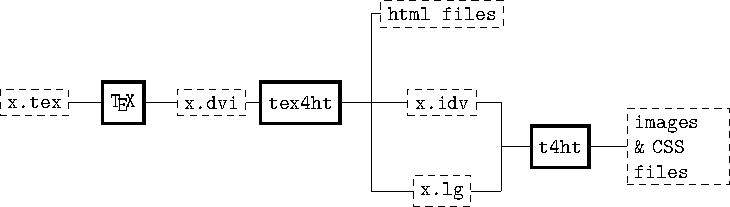
\includegraphics[width=\textwidth]{img/tex4ht_process.pdf}
\caption{\texfourht\ process overview}
\label{fig:overview}
\end{figure*}




\end{document}
